\documentclass[conference]{IEEEtran}

\usepackage[utf8]{inputenc}
\usepackage{graphicx}
\usepackage{xcolor}
\usepackage{booktabs}
\usepackage{url}
\usepackage{array}

\title{Spotify Listening Behavior Analysis Using Audio Features and Machine Learning}

\author{
\IEEEauthorblockN{Ayse Gulcan Yoruk}
\IEEEauthorblockA{DSA 210 Introduction to Data Science\\
Spring 2026}
}

\begin{document}
\maketitle

\begin{abstract}
This project analyzes a personal Spotify listening history enriched with Spotify audio features to study music preferences, listening patterns, and repeated listening behavior. Milestone 1 focused on exploratory data analysis and non-parametric hypothesis testing. Milestone 2 extends the project with a reproducible machine learning workflow that predicts whether a track is frequently played using audio features and selected Spotify metadata. The workflow uses leakage-aware preprocessing, stratified train/test splitting, cross-validated hyperparameter tuning, and model comparison across traditional classifiers. \textcolor{red}{TODO: Add the final best model, test F1-score, and key interpretation after rerunning milestone2.ipynb with the private data file.}
\end{abstract}

\section{Introduction / Motivation}
Music listening behavior can reflect personal preferences, mood, routines, and repeated engagement with specific artists or tracks. Spotify listening history provides a rich opportunity to analyze these patterns using both behavioral data and audio features. This project investigates whether Spotify audio features such as energy, valence, danceability, tempo, acousticness, and loudness can help explain listening patterns and predict whether a track is repeatedly played.

The project is designed as an academically honest and reproducible DSA 210 data science workflow. The raw listening history is private and therefore excluded from GitHub. Code, documentation, figures, and report scaffolding are included so the analysis can be reproduced locally by placing the private JSON file in the project root.

\section{Data Source}
The dataset consists of personal Spotify Extended Streaming History records enriched with Spotify Web API audio features. The private data file is expected to be named \texttt{gulcan\_spotify\_formatted.json}. Milestone 1 outputs report 1,558 play events, 1,535 unique tracks, and 921 unique artists covering April 2025 to April 2026.

\textcolor{red}{TODO: Confirm the exact data export date and describe the Spotify API enrichment process in more detail if required by the final course report.}

\section{Data Collection}
The listening records include track name, artist name, playback timestamp, and audio features. The raw JSON file is excluded from version control because it contains personal listening history. The repository includes notebooks and generated figures, but not the private raw data.

\section{Data Preprocessing}
The Milestone 2 notebook implements a preprocessing workflow using scikit-learn pipelines. Numeric variables are checked for missing values and skewness. Strongly skewed positive numeric variables are selected from the training split only and transformed using \texttt{log1p}. Numeric variables are imputed and scaled inside the model pipeline. Binary categorical variables such as Spotify mode are imputed and passed as binary values. Non-binary categorical variables such as Spotify key are one-hot encoded.

Track and artist text fields are detected and normalized through lowercase conversion, punctuation removal, and stopword removal. However, these identity-like text fields are excluded from the primary predictive model because they may encourage memorization rather than a generalizable claim about audio features. Date/time variables are engineered for analysis but excluded from the main model input to reduce leakage from listening opportunity.

\section{Exploratory Data Analysis}
Milestone 1 visualizations show distributions of Spotify audio features, feature correlations, top artists and tracks, monthly activity, hourly activity, valence over time, and energy-valence relationships.

\begin{figure}[htbp]
\centering

\includegraphics[width=\linewidth]{../figures/feature_distributions.png}
\caption{Distribution of Spotify audio features in the listening history.}
\label{fig:feature_distributions}
\end{figure}

\begin{figure}[htbp]
\centering

\includegraphics[width=\linewidth]{../figures/correlation_heatmap.png}
\caption{Correlation heatmap for Spotify audio features.}
\label{fig:correlation_heatmap}
\end{figure}

\section{Hypothesis Testing}
Milestone 1 tested four hypotheses using non-parametric methods where appropriate. The analysis found no statistically significant evidence that high-energy songs were played more frequently than low-energy songs, and no significant seasonal difference in valence between summer and winter. The analysis found evidence that acoustic songs had lower tempo than non-acoustic songs and that energy and danceability were positively correlated.

\begin{table}[htbp]
\centering
\caption{Milestone 1 hypothesis test summary.}
\begin{tabular}{p{0.35\linewidth}p{0.28\linewidth}p{0.14\linewidth}p{0.15\linewidth}}
\toprule
Hypothesis & Test & p-value & Result \\
\midrule
High-energy songs are played more & Mann-Whitney U & 0.8707 & Not rejected \\
Higher valence in summer & Mann-Whitney U & 0.8250 & Not rejected \\
Acoustic songs have lower tempo & Mann-Whitney U & $<0.0001$ & Rejected \\
Energy and danceability are positively correlated & Spearman rho & $<0.0001$ & Rejected \\
\bottomrule
\end{tabular}
\label{tab:hypothesis_summary}
\end{table}

\section{Machine Learning Methods}
Milestone 2 frames the problem as binary classification. A track is labeled as frequently played if its play count is at least two. The primary feature set includes audio features and selected Spotify metadata while excluding leakage-prone fields such as play count, first play time, last play time, track name, artist name, and text metadata.

The notebook evaluates Logistic Regression, Gaussian Naive Bayes, Decision Tree, Random Forest, Support Vector Machine, Gradient Boosting, and AdaBoost. Hyperparameters are tuned using cross-validation with a stratified split. If class imbalance is detected, F1-score is used as the primary tuning metric; otherwise accuracy is used.

\section{Results}
\textcolor{red}{TODO: Rerun milestone2.ipynb with gulcan\_spotify\_formatted.json and insert the final model comparison table.}

\begin{figure}[htbp]
\centering
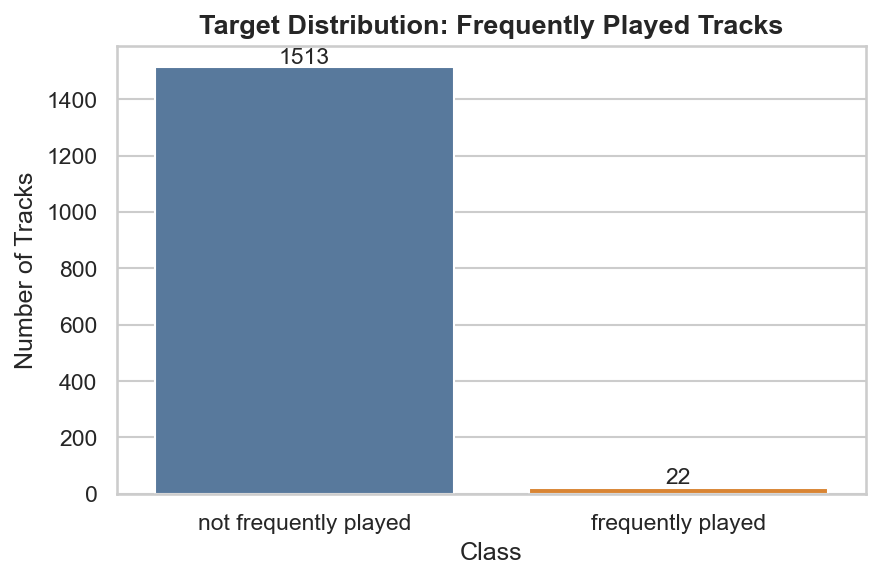
\includegraphics[width=\linewidth]{../figures/target_distribution.png}
\caption{Target distribution for the frequently played binary classification task.}
\label{fig:target_distribution}
\end{figure}

\begin{figure}[htbp]
\centering
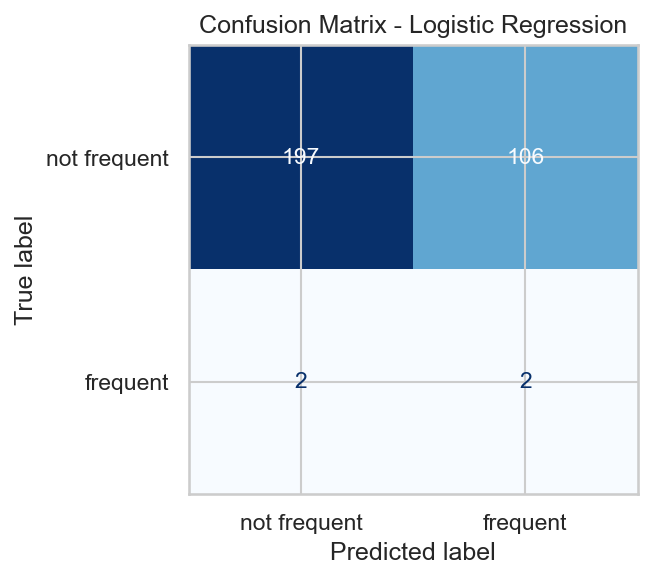
\includegraphics[width=\linewidth]{../figures/confusion_matrix_logistic_regression.png}
\caption{Confusion matrix for the tuned Logistic Regression classifier.}
\label{fig:cm_lr}
\end{figure}

\begin{figure}[htbp]
\centering
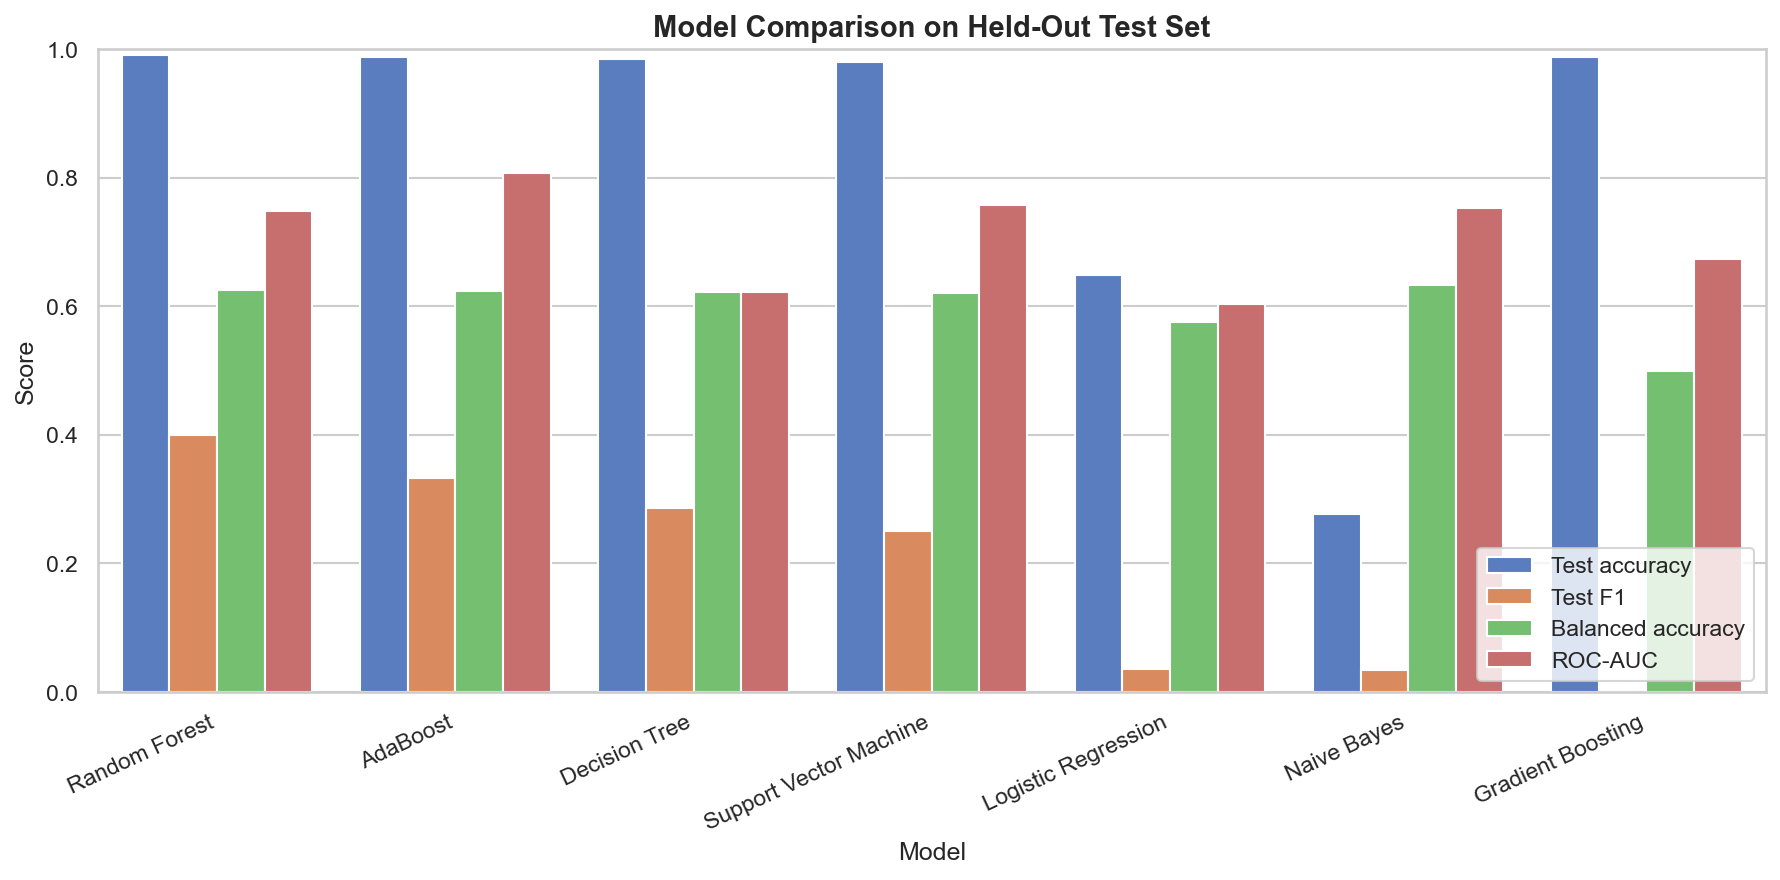
\includegraphics[width=\linewidth]{../figures/model_comparison.png}
\caption{Comparison of tuned machine learning models on the held-out test set.}
\label{fig:model_comparison}
\end{figure}

\begin{figure}[htbp]
\centering
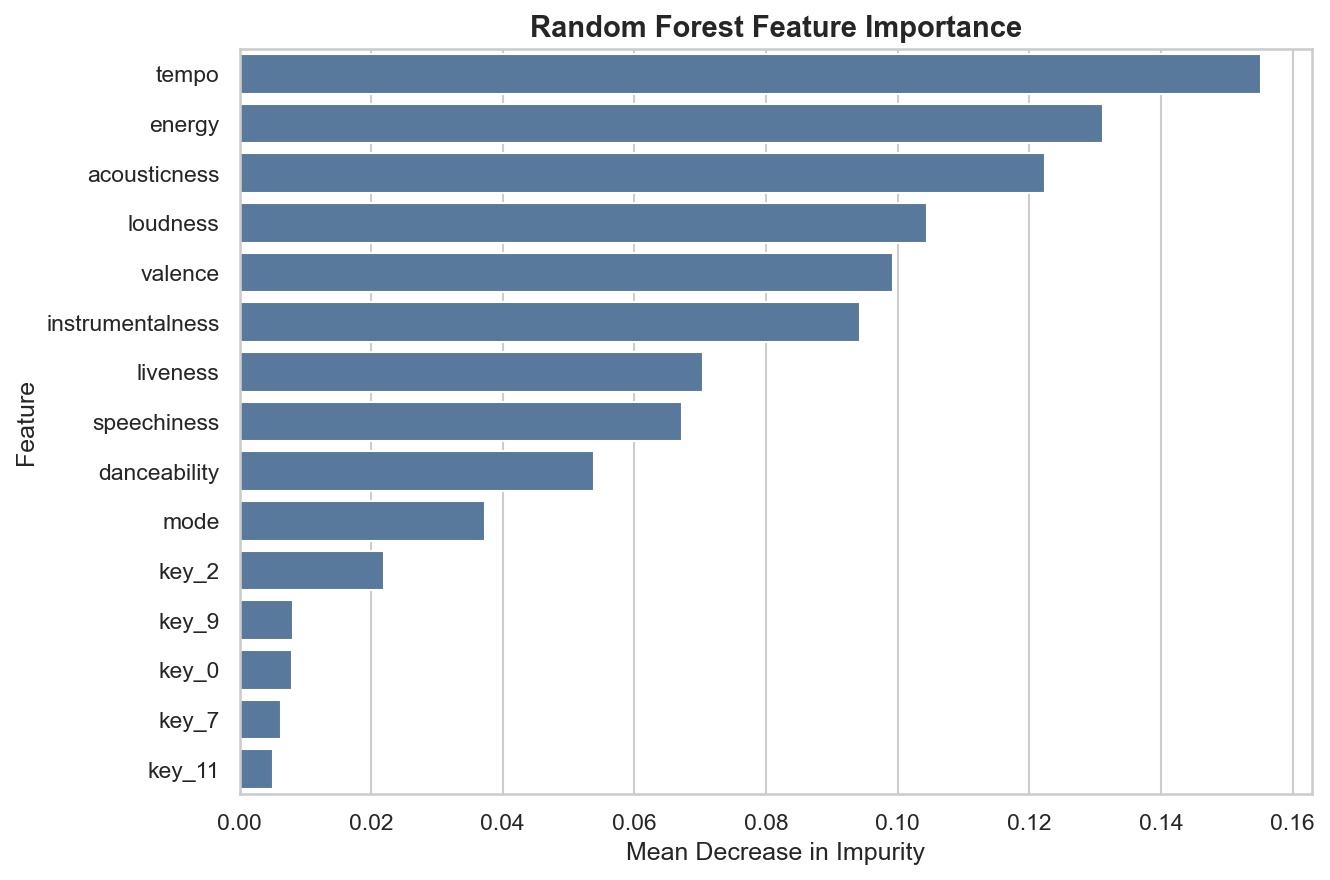
\includegraphics[width=\linewidth]{../figures/feature_importance_random_forest.png}
\caption{Random Forest feature importance for the primary audio-feature model.}
\label{fig:rf_importance}
\end{figure}

\section{Discussion}
\textcolor{red}{TODO: Add discussion after confirming the best model and its held-out test performance. Discuss whether audio features alone provide enough signal for repeated listening behavior.}

\section{Limitations}
The project uses one person's listening history, so findings should not be generalized to broader Spotify users. The target variable is based on repeated listening within the available history and may be affected by time window length, playlist behavior, mood, seasonality, and external context. Audio features alone may not capture social, lyrical, cultural, or situational reasons for repeated listening.

\section{Future Work}
Future work could evaluate temporal validation, include additional context features, compare audio-only models with carefully controlled text or artist-level baselines, and analyze model stability across different target thresholds such as three or more plays.

\section{Ethical Considerations}
The raw data contains personal listening history and is therefore excluded from the public repository. The analysis should avoid overclaiming psychological or emotional conclusions from audio features alone. Any sharing of the project should preserve privacy and avoid exposing personally sensitive listening records.

\section{AI Assistance Disclosure}
AI assistance was used to improve project organization, preprocessing design, machine learning pipeline structure, repository documentation planning, and this LaTeX scaffold. The assistance did not fabricate data or model results. Unverified results are marked with red TODO notes until the notebook is rerun with the private data file. This section is the project's AI assistance disclosure.

\section{References}
\begin{thebibliography}{1}
\bibitem{spotify}
Spotify for Developers, ``Web API Reference,'' \url{https://developer.spotify.com/documentation/web-api}.

\bibitem{sklearn}
F. Pedregosa et al., ``Scikit-learn: Machine Learning in Python,'' Journal of Machine Learning Research, vol. 12, pp. 2825--2830, 2011.

\bibitem{scipy}
P. Virtanen et al., ``SciPy 1.0: Fundamental Algorithms for Scientific Computing in Python,'' Nature Methods, vol. 17, pp. 261--272, 2020.

\bibitem{course}
\textcolor{red}{TODO: Add the official DSA 210 project guideline reference if a citation format is required.}
\end{thebibliography}

\end{document}
